\documentclass{article}

% if you need to pass options to natbib, use, e.g.:
% \PassOptionsToPackage{numbers, compress}{natbib}
% before loading nips_2016
%
% to avoid loading the natbib package, add option nonatbib:
% \usepackage[nonatbib]{nips_2016}

\usepackage[final]{nips_2016}

% to compile a camera-ready version, add the [final] option, e.g.:
% \usepackage[final]{nips_2016}

\usepackage[utf8]{inputenc} % allow utf-8 input
\usepackage[T1]{fontenc}    % use 8-bit T1 fonts
\usepackage{hyperref}       % hyperlinks
\usepackage{url}            % simple URL typesetting
\usepackage{booktabs}       % professional-quality tables
\usepackage{amsfonts}       % blackboard math symbols
\usepackage{nicefrac}       % compact symbols for 1/2, etc.
\usepackage{microtype}      % microtypography
\usepackage{amsmath}		% math library
\usepackage{graphicx}
\usepackage{caption}
\usepackage{subcaption}
\graphicspath{{./images/}}

\title{Voxel-wise nonlinear analysis toolbox for neurodegenerative diseases and aging}

% The \author macro works with any number of authors. There are two
% commands used to separate the names and addresses of multiple
% authors: \And and \AND.
%
% Using \And between authors leaves it to LaTeX to determine where to
% break the lines. Using \AND forces a line break at that point. So,
% if LaTeX puts 3 of 4 authors names on the first line, and the last
% on the second line, try using \AND instead of \And before the third
% author name.

\author{
  Authors\\
  Signal Theory and Communications Department\\
  Universitat Politècnica de Catalunya, BarcelonaTech\\
  Barcelona, Spain \\
  \texttt{email}\\
  %% \AND
  %% Coauthor \\
  %% Affiliation \\
  %% Address \\
  %% \texttt{email} \\
  %% \And
  %% Coauthor \\
  %% Affiliation \\
  %% Address \\
  %% \texttt{email} \\
  %% \And
  %% Coauthor \\
  %% Affiliation \\
  %% Address \\
  %% \texttt{email} \\
}

\begin{document}
% \nipsfinalcopy is no longer used

\maketitle

\begin{abstract}
  The abstract paragraph should be indented \nicefrac{1}{2}~inch
  (3~picas) on both the left- and right-hand margins. Use 10~point
  type, with a vertical spacing (leading) of 11~points.  The word
  \textbf{Abstract} must be centered, bold, and in point size 12. Two
  line spaces precede the abstract. The abstract must be limited to
  one paragraph.
\end{abstract}

\section{Introduction}

\section{The toolbox}
\label{toolbox}

The toolbox comprises an independent \textit{fitting library}, made up of different \textit{model fitting} and \textit{fit evaluation} methods, a \textit{processing} module that interacts with the aforementioned \textit{fitting library} providing the formatted data obtained from the \textit{file system}, several \textit{visualization} tools and a \textit{CLI interface} that allows the interaction between the user and the \textit{processing} module, supported by a \textit{configuration file}. 

\subsection{Model fitting techniques}

A model fitting consists on finding a parametric or a nonparametric function of some explanatory variables (\textbf{predictors}) and possibly some confound variables (\textbf{correctors}) that best fits the observations of the target variable in terms of a given quality metric or, conversely, that minimizes the loss between the prediction of the model and the actual observations.
\begin{itemize}
\item \textbf{General Linear Model (GLM)} 

The General Linear model is a generalization of multiple linear regression to the case of more than one dependent variable. 
A possible approach to model nonliniearities with this model is a polynomial basis expansion of degree $d$, that is, the input space $\mathfrak{X}$ is mapped into another feature space $\mathfrak{F}$ that also includes the polynomial terms of the variables: ($\Phi : \mathfrak{X} \rightarrow \mathfrak{F}$).

\item \textbf{Generalized Additive Model (GAM)} 

A Generalized Additive Model is a Generalized Linear Model in which the observations of the target variable depend linearly on unknown smooth functions of some predictor variables: $ f(X) = \alpha + \sum_{i=1}^{k} f_i(X_i)$. Here $f_1, f_2, ..., f_k$ are nonparametric smooth functions that are simultaneously estimated using scatterplot smoothers by means of the \textbf{backfitting algorithm}. Several fitting methods can be accomodated in this framework by using different smoother operators, such as cubic splines, polynomial or Gaussian smoothers. 

\item \textbf{Support Vector Regression (SVR)} 

The regression counterpart of the well-known Support Vector Machines, Support Vector Regression, is based on the following idea: the goal is to find a function that has at most $\epsilon$ deviation from the observations and, at the same time, is as flat as possible. However, the $\epsilon$ deviation contraint is not feasible sometimes, and a hyperparameter that controls the degree up to which deviations larger than $\epsilon$ are tolerated is introduced, $C$. 
In the context of SVR nonlinearities are introduced with the "kernel trick", that is, a kernel function $ k(x_i, x_j) = \langle \Phi(x_i), \Phi(x_j) \rangle $ is introduced that implicitly maps the inputs from their original space into another high-dimensional space without requiring to know the explicit mapping $ \Phi(\cdot) $. 
The kernel function used in this toolbox is the Radial Basis Function or Gaussian kernel, which is defined as $ k(x_i, x_j) = exp(-\gamma \|x_i - x_j\|^2)$.
\end{itemize}

\subsection{Hyperparameters search algorithm}

Support Vector Regression methods rely on several hyperparameters, namely $\epsilon$ and $C$ in general and also $\gamma$ when using a RBF kernel function. To address the search of these hyperparameters an automatic method based on grid search is included in this toolbox, which comprises the following steps: 1) sample the hyperparameters space in a grid using one of the several sampling methods provided in the toolbox; 2) fit a subset of the data with the combination of hyperparameters of each sample in the grid; 3) select the combination that minimizes the error function of choice. 

The lack of validation data and the nature of morphometric data, which is vastly dominated by voxels with 0-valued observations, limits the ability to find a subset of the data that is valid to find the optimal hyperparameters without incurrying in overfitting or underfitting. For that reason the following approach is taken: a subset of $m$ voxels is selected in each of the $N$ iterations of the algorithm, the $m$ selected voxels must contain observations with a minimum variance of $Var_{min}$, and the error computed for each voxel is weighted by the inverse of the variance of its observations. 


\subsection{Fit evaluation methods}
\begin{itemize}
	
\item \textbf{MSE}, \boldmath{$R^2$}

Well known metrics that evaluate the predictive power of the model but don't penalize its complexity.

\item \textbf{Akaike Information Criterion (AIC)}

Criterion based on information theory widely used for model comparison and selection. Unlike the previous ones, it does penalize the complexity of the model by requiring its number of parameters $k$.

\item \textbf{F-test} 

The F-test evaluates whether the variance of the full model (correctors and predictors) is significantly lower — from a statistical point of view — than the variance of the restricted model (only correctors), that is, the inclusion of the predictors contributes to the explanation of the observations. 
This statistical test requires the degrees of freedom of both models, which are trivial to compute in GLM, but they aren't in GAM or SVR. The equivalent degrees of freedom for Support Vector Regression were introduced in the toolbox as defined in \ref{}.

\item \textbf{PRSS\footnote{Penalized Residual Sum of Squares}, Variance-Normalized PRSS} 

Penalized Residuals Sum of Squares is introduced in the toolbox in order to provide a fit evaluation metric that penalizes the complexity of the predicted curve without requiring the degrees of freedom. However, PRSS is not suitable enough in the context of morphometric analysis, as it always provides better scores for target variables with low-variance and flat trends than for target variables with high-variance and nonflat trends, and that poses a problem as most of the voxels in the brain are 0-valued. 

For that reason a variance normalized version of the PRSS that weights the score with the inverse of the variance of the predicted curve was introduced, the Variance Normalized Penalized Residuals Sum of Squares.

\end{itemize}

\subsection{Interactive visualization tool}

An interactive visualization tool is included in the toolbox to provide added insight on the results: it allows to load a 3D statistical map — generated with the fit evaluation method of choice — and several fitted models, and then plots the predicted curves of all the models for the voxel selected with the cursor, hence easing the task of inspecting the curves in the significant regions. An example of the aforementioned tool is found in \autoref{fig:vnprss_high_fitscore_curve_apoe}. 

\section{Implementation details}

The whole toolbox has been implemented in Python. Numpy and scipy have been used for the numerical and scientific computing, NiBabel for handling the morphometric data in NIfTI format, scikit-learn for the machine learning algorithms and matplotlib and seaborn for plotting and for the visualization features.

\section{Dataset}

\section{Experiments}

\begin{figure}[!htp]
	\centering
	\begin{minipage}{.45\textwidth}
		\centering
		\captionsetup{justification=centering,margin=0.5cm}
		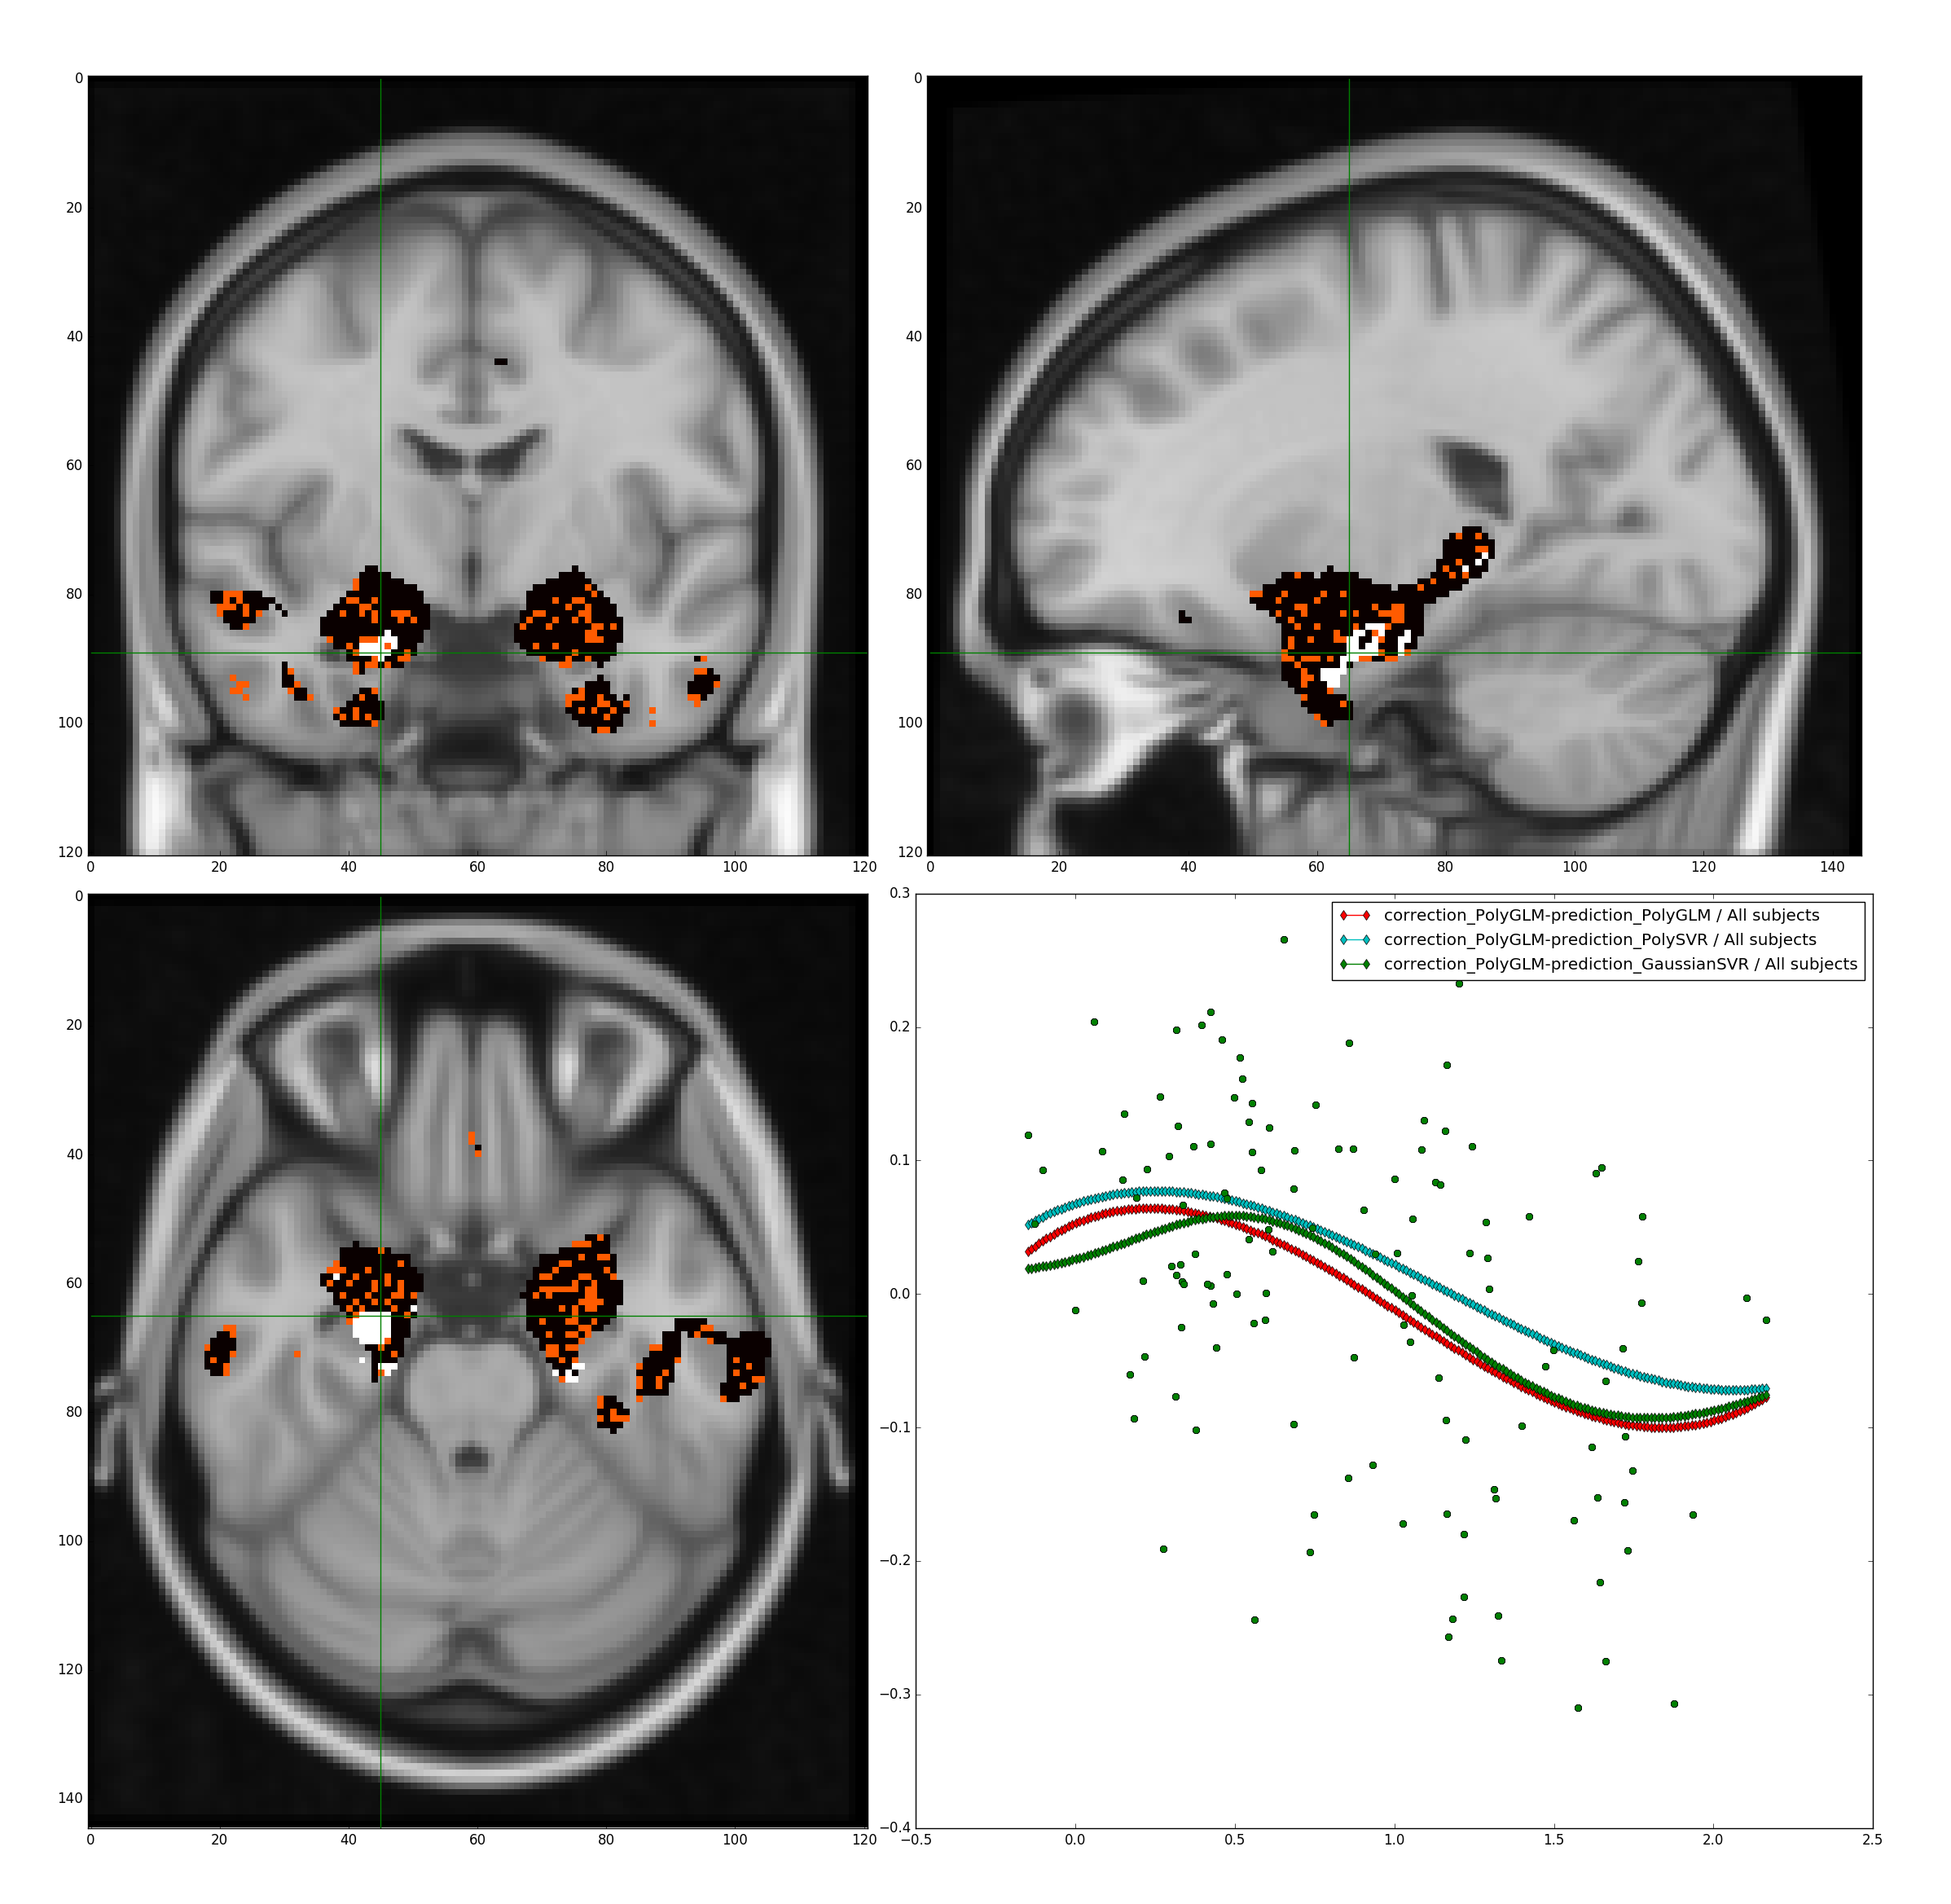
\includegraphics[width=.95\linewidth]{gvis_best_gsvr_vs_pglm_vs_psvr.png}
		\captionof{figure}{\textit{BEST} model of polynomial GLM vs polynomial SVR vs Gaussian SVR with the corresponding curves for a voxel in which the best fitting score belongs to the Gaussian SVR model.}
		\label{fig:gsvr_best}
	\end{minipage}
	\begin{minipage}{.45\textwidth}
		\captionsetup{justification=centering,margin=0.5cm}
		\centering
		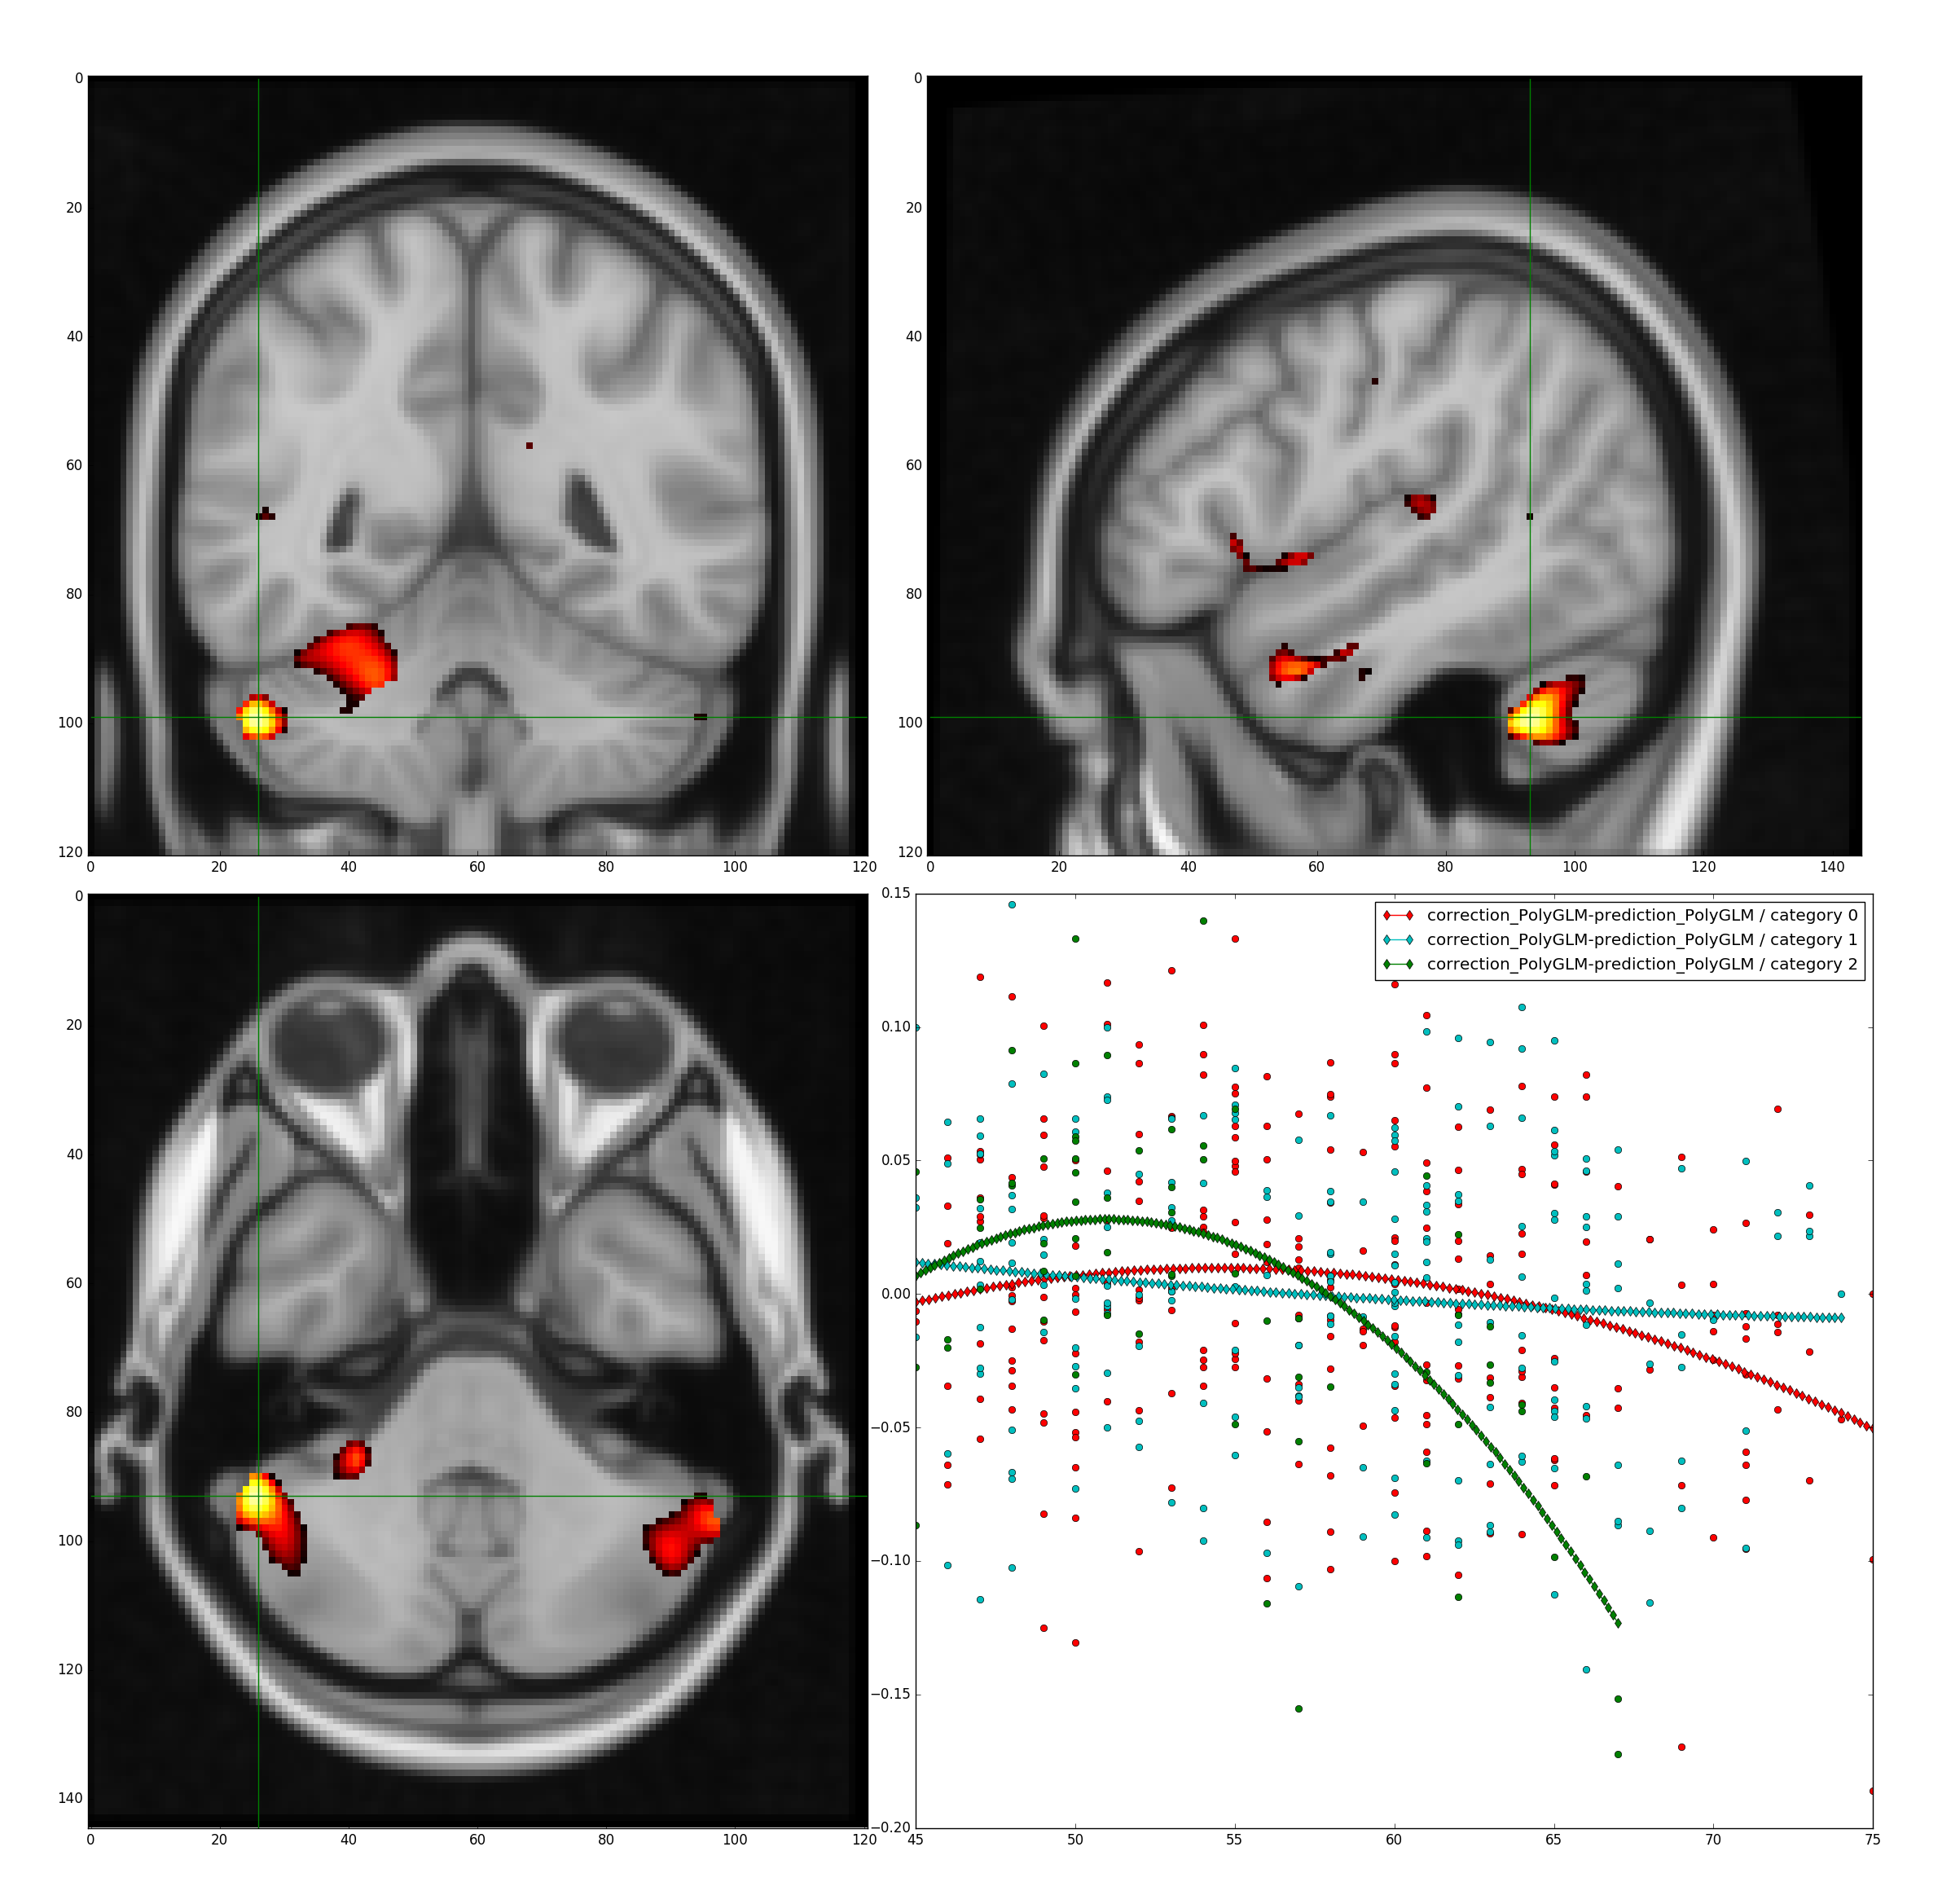
\includegraphics[width=.95\linewidth]{vnprss_high_fitscore_curve.png}
		\captionof{figure}{VN-PRSS statistical map for the polynomial model in \textit{Aging atrophy with regards to the APOE4 genotype} problem and the associated curve in a voxel with a high fit score.}
		\label{fig:vnprss_high_fitscore_curve_apoe}
	\end{minipage}%
\end{figure}

Sample figures.

\section{Conclusions}

\subsubsection*{Acknowledgments}


\section*{References}
\small

[1] Alexander, J.A.\ \& Mozer, M.C.\ (1995) Template-based algorithms
for connectionist rule extraction. In G.\ Tesauro, D.S.\ Touretzky and
T.K.\ Leen (eds.), {\it Advances in Neural Information Processing
  Systems 7}, pp.\ 609--616. Cambridge, MA: MIT Press.

\end{document}
